\section{Translating kernel outputs as inputs to higher-order layers}

%%%%%%%%%%%%%%%%%%%%%%%%%%%%%
\begin{figure*}[htb]
\centering
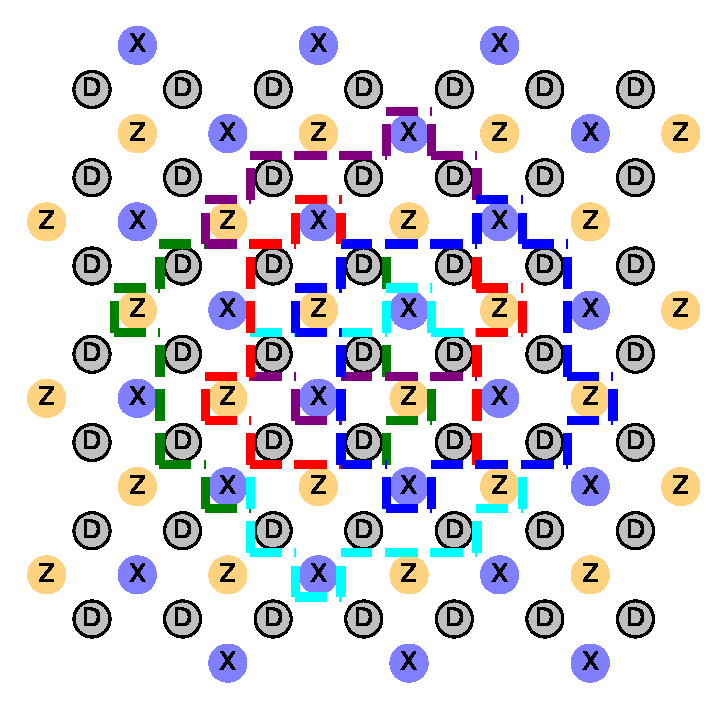
\includegraphics[width=0.6\textwidth]{d7_q25_kernels.pdf}
\ccaption
{$d=3$ kernels surrounding a data qubit in a $d=7$ surface code}
{
}
\label{fig:d7wkern}
\end{figure*}
%%%%%%%%%%%%%%%%%%%%%%%%%%%%%

In the example shown for a $d=7$ code in Fig.~\ref{fig:d7wkern}, all of the displayed kernels are of the same unique type. We highlight the central red kernel as a standard $d=3$ surface code patch and the blue one corresponding to its flipped counterpart. For simplicity, we will number all data qubits from 1 (top left) to 7 (top right) and 49 (bottom right) and denote the corresponding qubit numbers on the kernel patch with a prime indicator, \eg, qubit 18 $\rightarrow$ \kernum{2} in the red kernel and \kernum{3} in the blue one.

Kernels assume uniform noise to maximize the number of weights shared. Symmetries are broken in kernel types that evaluate et the boundary of the surface code. For that reason, all of the weights become unique, and these kernels have 9 outputs. In the only kernel type that does not evaluate at any boundary, only the weights that are associated with kernel qubits \kernum{1}, \kernum{2}, \kernum{3}, \kernum{5}, \kernum{6}, and \kernum{9} are unique, and this kernel has 6 outputs instead of 9.

The kernels displayed in Fig.~\ref{fig:d7wkern} surround qubit 25, the only qubit that can be shared exclusively by kernels of the last type, and we will use this qubit as an example to explain the translation of kernel outputs. Here, the nine kernels colored in red, blue, dark green, magenta, cyan, pink, light green, brown, and orange contribute to the prediction for an error in this qubit with outputs that correspond to kernel qubit positions \kernum{5}, $\kernum{4}\equiv\kernum{6}$, \kernum{6}, $\kernum{8}\equiv\kernum{2}$, \kernum{2}, $\kernum{9}\equiv\kernum{1}$, $\kernum{7}\equiv\kernum{3}$, \kernum{3}, and \kernum{1} respectively. For that reason, these contributions can be encoded as a list of ordered pairs of integers as $\{(5,1)^2, (5,2)^2, (5,3)^2, (5,5), (5,6)^2\}$, with the first integer in each pair corresponding to the unique type of the contributing kernel, the second one marking the contributing kernel qubit position, and the exponent indicating the number of occurrence of this pair. The number of such unique contributions and the total count of associated parameters are listed in Table~\ref{table:unique-kern-contribs}.

%%%%%%%%%%%%%
\begin{table}[htbp]
\centering
\ccaption
{Parameter counts to combine kernels}
{
The counts are listed separately for kernel sizes $k=3$ and $k=5$ over distance-$d$ surface codes.
The numbers $C$ refer to the total number of unique combinations of kernel contributions to each of the $d^2$ data qubits.
For any odd kernel size $k$, the values of $C$ begin to alternate with the same values for odd and even $d$ above $d=2k+1$, \ie, $d=7$ for $k=3$ and $d=11$ for $k=5$.
For smaller distances, $C=(d/2)^2$ for even and $(d^2+1)/2$ for odd $d$ values.
The composition of the unique combinations determines the number of fraction and phase parameters needed in the NN,
with the number of fractions reported for the recursive parametrization method described in the main text.
}
\renewcommand{\arraystretch}{1.25}
\begin{tabular}{c ccc ccc}
\hline
      & \multicolumn{3}{c}{$k=3$}   & \multicolumn{3}{c}{$k=5$} \\
\hline
$d$ & ~~~$C$ & Fractions & Phases & ~~~$C$ & Fractions & Phases \\
\hline
4 & ~~~4 & 5 & 8 & ~~~- & - & - \\
5 & ~~~13 & 28 & 62 & ~~~- & - & - \\
6 & ~~~9 & 27 & 80 & ~~~9 & 16 & 28 \\
7 & ~~~25 & 86 & 262 & ~~~25 & 88 & 272 \\
8 & ~~~16 & 59 & 182 & ~~~16 & 84 & 400 \\
9 & ~~~25 & 86 & 262 & ~~~41 & 268 & 1504 \\
10 & ~~~16 & 59 & 182 & ~~~25 & 194 & 1272 \\
11 & ~~~25 & 86 & 262 & ~~~61 & 522 & 3554 \\
12 & ~~~16 & 59 & 182 & ~~~36 & 328 & 2282 \\
\hline
\label{table:unique-kern-contribs}
\end{tabular}
\end{table}



If each output of a kernel is bounded between 0 and 1, through sigmoid activation, and can loosely be interpreted as a probability $p_i$ for an error, the combined prediction can be written through the reparametrization $x_i=\sqrt{\frac{p_i}{1-p_i}}$. Using an analogy to write the magnitude of a complex number from a sum of two others, the parameter $x$ for the combined probability can therefore be expressed as
\begin{equation}
\begin{aligned}
S_i &= \sum_{k_i=1}^{n_i} f_i x^2_{k_i}, \\
x^2 &= \sum_{i=1}^{N} \left( S_i + 2 \sum_{j=i+1}^{N} \sqrt{S_i S_j} \cos{\phi_{ij}} \right).
\end{aligned}
\label{eq:kernsum}
\end{equation}
Here, the indices $i$ and $j$ run over a total of $N$ unique combinations of kernel type--kernel qubit index pairs, \eg, $N=5$ for qubit 25, and the indices $k_i$ run over the evaluations of this unique combination $i$ in $n_i$ different strides, \eg, for contribution type $(5,5)$ to qubit 25, $k_i$ can only be 1, but it runs up to $n_i=2$ for all other contribution types.

In constructing $S_i$, we assume that evaluations of the same combination $i$ have an underlying complex representation with the same overall phase, but $S_i$ values with different indices $i$ do not have to carry the same phase, which justifies the phase difference parameters $\cos{\phi_{ij}}$.
The fractions $f_i$ are subject to the constraint $\sum_{i=1}^{N} f_i = 1$, so they can be parametrized using recursive fractions, which would satisfy the constraint by construction and avoid a spurious parameter, \ie, through the mapping $f_1 \to f_1$, $f_i \to f_i\prod_{j=1}^{i-1}\left(1-f_j\right)$ for $1<i<N$, and $f_N \to \prod_{j=1}^{N-1}\left(1-f_j\right)$. Both these fractions and the phase parameters $\cos{\phi_{ij}}$ are included as unique sets of weights between 0 and 1 to be determined during NN training.

The final probability $p$ computed from the output of all kernels could simply be found from the inverse transformation on $x$, \ie, $p=\frac{x^2}{1+x^2}$, but as a further input to the higher hierarchy of layers, we keep it untransformed as $x^2$. Since there are $d^2$ such values, corresponding to each physical data qubit, leaving $x^2$ as is adds flexibility for the NN to learn nonuniform noise at the level of higher layers.
